\documentclass{article}
\usepackage{graphicx} % Required for inserting images
\usepackage[margin=2.5cm]{geometry}
\usepackage[T1]{fontenc}
\usepackage{lmodern}
\usepackage{booktabs}
\usepackage{amsmath}
\usepackage{caption}
\usepackage{float}
\usepackage[hidelinks]{hyperref}

\graphicspath{{figures/}{./}}

\title{BodySync: A Personal Stress Score from Your Wristband}
\author{Swayam Lakhotia \and Ananya Khaitan \and Bhavya Bajaj}
\date{November 2026}

\begin{document}
\maketitle

\section{The idea}

Wristbands like the Empatica record heart rate, sweat (EDA) and skin temperature all day. Sun et al.~\cite{sun2026trust} showed that these signals react when people are under pressure, but analysed each signal separately, in a single lab session. \textbf{BodySync} turns them into one 0--100 score for everyday use: 100 means your body is at \emph{its own} normal, and lower means it is reacting the way it does under stress.

Everyone's normal is different, so BodySync compares you only with yourself, never with other people.

\section{What we tried first}

Our first idea was that stress throws the body \emph{out of step}: normally heart rate, sweat and skin temperature rise and fall together in a person's usual way, and stress might break that pattern (``sync''). For every 30-minute window we computed the correlation between each pair of signals (heart rate--sweat, heart rate--temperature, sweat--temperature) and compared it with that person's usual correlation.

We checked this idea in two ways:
\begin{itemize}
\item \textbf{Does sync carry any information?} On an everyday dataset of 27 people who wore an Empatica wristband for several days, a model given only the three sync values had to tell asleep, resting (awake and still) and active apart, using the watch's own labels and testing each person on a model trained on the others. It was right 37\% of the time, where random guessing gets 33\%.
\item \textbf{Does it see stress?} On the WESAD lab study, a sync score picked out stress 0.46 of the time, where 0.5 is a coin flip.
\end{itemize}

The signals stayed in step whether people were stressed or calm. What did change under stress was their \emph{level}: heart rate and sweat went up and the skin cooled, compared with that person's usual values. So the final BodySync measures how far each signal is from a person's own normal, not how the signals move together.

\section{How BodySync works}

\begin{enumerate}
\item \textbf{Your normal.} Each person's usual heart rate, sweat and temperature.
\item \textbf{Stress signals,} measured against that normal: sweat bursts (small, fast spikes in sweat, which jump from about 2 to about 10 per minute under stress), the fast and slow parts of the sweat signal, whether heart rate and temperature are rising or falling, and how much each changed over the last 10 minutes.
\item \textbf{A trained model} combines these, then adapts to each person using their own unlabelled days (self-training).
\item \textbf{The score} is smoothed over the last few minutes, since stress lasts minutes, not seconds.
\end{enumerate}

\subsection*{The first version: a plain formula}

The first version of the personal-normal score (``first version'' below) has no learning. For each signal $i$ (heart rate, sweat, skin temperature), it measures how far the current value $x_i$ is from that person's normal, in units of their usual spread. This is a z-score:
\[
z_i = \frac{x_i - \mathrm{normal}_i}{\mathrm{spread}_i},
\]
where the normal is the person's median and the spread is a robust standard deviation (the median absolute deviation, times 1.48, so that a few odd moments do not inflate it). Sweat is used on a log scale, because it varies hugely between people, and each spread has a small minimum (2 bpm for heart rate, 0.1\,\textdegree C for temperature) so that very steady people do not get huge z-scores from tiny changes.

Only the stress direction counts: heart rate up, sweat up, temperature \emph{down}. A heart rate below normal or warmer hands is not stress, so those count as zero ($z_i^+ = \max(0, z_i)$, with the sign of temperature flipped). The three are combined into one distance and turned into a score:
\[
d = \sqrt{\tfrac{1}{3}\left( (z^+_{\mathrm{HR}})^2 + (z^+_{\mathrm{sweat}})^2 + (z^+_{\mathrm{temp}})^2 \right)}, \qquad \mathrm{score} = \frac{100}{1 + d/2}.
\]

\begin{table}[H]
\centering\small
\caption{A worked example. Heart rate and sweat are both two spreads above normal; temperature is at normal.}
\begin{tabular}{lcccc}
\toprule
Signal & Normal & Spread & Now & $z^+$ \\
\midrule
Heart rate & 70 bpm & 5 bpm & 80 bpm & $(80-70)/5 = 2$ \\
Sweat & usual level & usual spread & 2 spreads above & 2 \\
Skin temperature & usual level & usual spread & at normal & 0 \\
\midrule
\multicolumn{5}{l}{$d = \sqrt{(2^2 + 2^2 + 0^2)/3} \approx 1.63$, \quad score $= 100/(1 + 1.63/2) \approx 55$} \\
\bottomrule
\end{tabular}
\end{table}

At your normal $d = 0$ and the score is 100; one spread away gives 67, two give 50 and six give 25. The score never reaches 0.

\subsection*{The final version: a model that learns, then tunes itself to you}

The final BodySync keeps the same idea (everything is measured as a distance from the person's own normal) but replaces the fixed formula with a trained model. Its inputs are the distances for heart rate, sweat and temperature, plus sweat bursts, heart-rate variability, the fast and slow parts of the sweat signal, whether heart rate and temperature are rising or falling, and how much each changed over the last 10 minutes. The model is XGBoost: many small decision trees whose votes are added up. Because it only ever sees distances from each person's normal, one model works for everyone.

\textbf{Self-training} then tunes it to each new person without any stress answers: the model scores all of that person's unmarked time, takes the 10\% of moments that look most stressed and the 10\% that look calmest as extra ``stress'' and ``calm'' examples, retrains once, and scores the person again. Weighting these examples more, or retraining continuously as new data comes in, did not help further.

\section{Data}

\begin{table}[H]
\centering\small
\caption{Datasets. Citation counts from OpenAlex, November 2026.}
\begin{tabular}{llrrl}
\toprule
Dataset & Setting & People & Citations & Stress label \\
\midrule
WESAD~\cite{wesad} & lab & 15 & 1{,}352 & speech + maths test \\
AffectiveROAD~\cite{affectiveroad} (new) & real driving & 9 & 125 & city traffic vs highway \\
Stress-Predict~\cite{stresspredict} & lab & 35 & 113 & Stroop test + interview \\
Stress + exercise~\cite{stressexercise} & lab & 36 & 37 & stress tasks + cycling \\
CAN-STRESS~\cite{canstress} & daily life & 62 & 1 & stress ratings 0--9 \\
\bottomrule
\end{tabular}
\end{table}

All five stress datasets use the same wristband, the Empatica E4.

\section{How we tested it}

\begin{itemize}
\item \textbf{Locked test people.} Before building the final system we set aside 40\% of the people in every dataset. All improvements were developed on the other 60\%, and the locked group was used once, at the very end. All results below are on them.
\item \textbf{Unseen people only.} Each test person is scored by a model that never saw their labels.
\item \textbf{The number.} For each person, take every pair of one stressed moment and one calm moment, and count how often the stressed one scores lower; then average over people. 0.5 is a coin flip and 1 means always (the within-person AUC). Because it is computed within each person, it cannot be fooled by one person simply having higher readings than another. So 0.90 means: pick a stressed and a calm moment from the same person, and the stressed one scores lower 9 times out of 10.
\item \textbf{Leak check.} With each person's stress labels scrambled, the final model scores 0.51 on average, a coin flip, so the gains are not an artefact.
\item \textbf{Shortcut checks.} In lab studies, stress can come with things that are not stress: talking and moving during the task, or always coming before the rest periods. The lab results hold with wrist movement removed from the model (WESAD 0.99+, Stress + exercise 0.91, Stress-Predict 0.88) and when rest periods right after a stressor are left out (0.99+, 0.91, 0.90). Timing is harder to rule out: in these studies stress always comes at the same point in the session, so a model given only the clock also scores high (WESAD 0.97, Stress-Predict 0.96, Stress + exercise 0.78). BodySync never sees the clock, but lab data alone cannot prove it is not partly tracking time; the driving test below does not have this problem.
\end{itemize}

\section{Results}

\begin{table}[H]
\centering\small
\caption{Locked test people: how well each version picks out stress (0.5 = coin flip, 1 = always).}
\begin{tabular}{llccc}
\toprule
Dataset & Setting & Test people & First version$^\dagger$ & Final BodySync \\
\midrule
WESAD$^*$ & lab & 6 & 0.92 & \textbf{0.99+} \\
Stress + exercise & lab & 14 & 0.63 & \textbf{0.91} \\
Stress-Predict & lab & 14 & 0.62 & \textbf{0.90} \\
CAN-STRESS & daily life & 10 & 0.59 & \textbf{0.67} \\
\midrule
Average & & & 0.69 & \textbf{0.87} \\
\bottomrule
\end{tabular}

\smallskip
\footnotesize $^\dagger$The plain formula above. $^*$Six test people; WESAD's speech and mental-arithmetic stressor is very strong, so even the plain formula scores 0.92.
\end{table}


\begin{figure}[H]
\centering
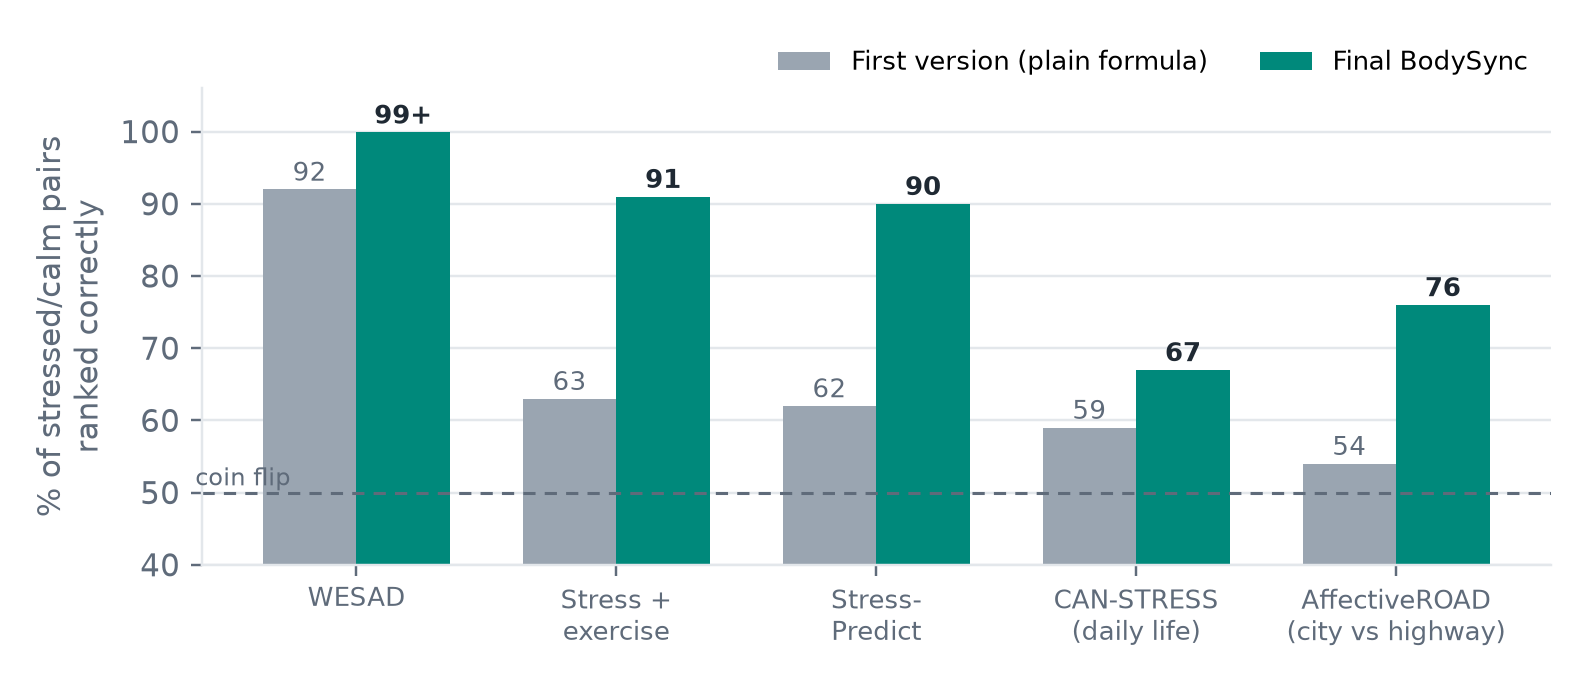
\includegraphics[width=\linewidth]{fig8_first_vs_final.png}
\caption{First version (plain formula) against the final BodySync, on people it never saw: the locked test people of the four main studies, and all nine drivers of AffectiveROAD (city vs highway, a dataset it never saw). The dashed line is a coin flip.}
\end{figure}

\paragraph{Lab stress.} The final BodySync picks out stress about 90\% of the time or better on every lab dataset, up from about 0.6 on the two harder ones. On Stress-Predict, all 14 test people scored lower under stress.

\paragraph{Everyday life.} On CAN-STRESS, the largest daily-life dataset, BodySync improves from 0.59 to 0.67. One caution: in CAN-STRESS the calm reports cluster in the evening, so time of day may explain part of this; too few people report stress and calm at matching hours to separate the two. Everyday stress is milder than a lab stress test and is only reported a few times a day, which makes it the hard part.

\paragraph{What helped.} Every idea was tried on the development people and kept only if it helped on average. Averaged over all five studies (the four main studies on the development people, plus real driving with a model that never saw it), the plain formula scored 0.56. A trained model lifted this to 0.69; sweat bursts added 0.035 (0.11 on WESAD and 0.09 on driving, but slightly less on Stress-Predict and CAN-STRESS); smoothing 0.01; fast and slow sweat 0.03; change over the last 10 minutes 0.03; and self-training, added last, 0.02 (0.08 on driving, 0.01 on CAN-STRESS), reaching 0.82. How much each step adds depends on the order, because steps overlap. Pooling all datasets, separate normals for still and moving, other model types, a normal built only from past days, and training on exactly the tested comparison did not help. Two later rounds aimed at everyday life (learning from all everyday datasets together; scoring only while still) helped on the development people but not consistently on two further, disclosed looks at the locked people, so the final system stays as above.

\begin{figure}[H]
\centering
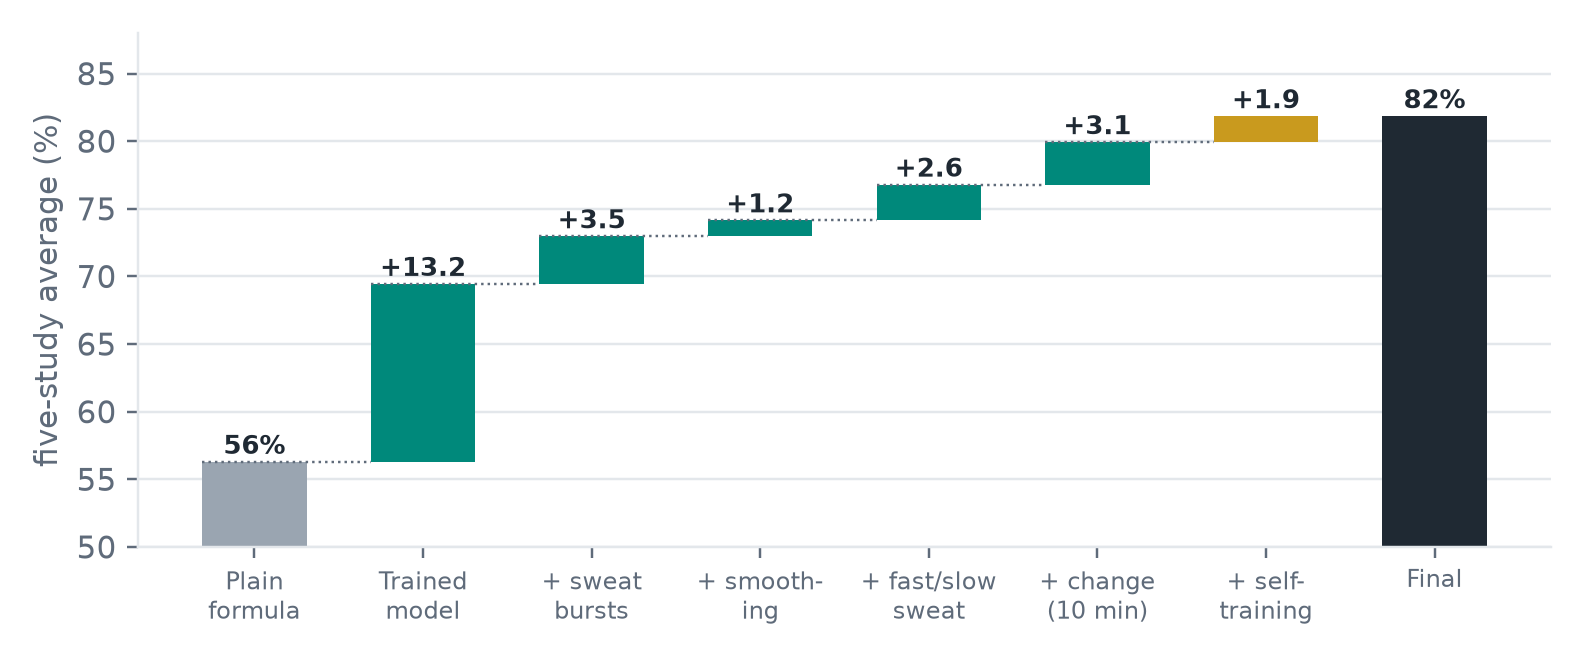
\includegraphics[width=\linewidth]{fig9_steps.png}
\caption{What each step added, in the order it was built, averaged over the five studies (the four main studies on the development people, plus driving). Self-training, in gold, is added last.}
\end{figure}

\begin{figure}[H]
\centering
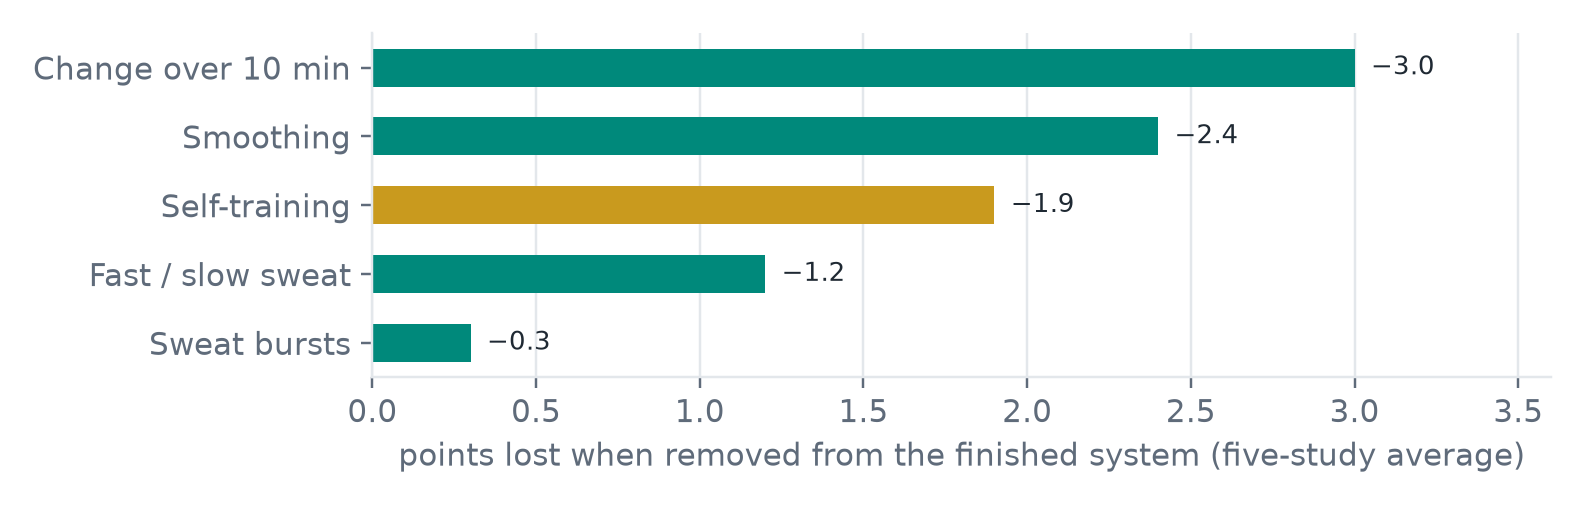
\includegraphics[width=\linewidth]{fig10_drop_one.png}
\caption{Taking one step out of the finished system at a time. The gain is spread out: no single step carries it, and sweat bursts matter little once the other sweat features are in.}
\end{figure}

\subsection*{A brand-new dataset: real driving}

After the final system was frozen we added AffectiveROAD~\cite{affectiveroad} from the MIT Media Lab: 9 drivers on 13 real drives through city traffic and on the highway, wearing the same Empatica wristband, with a 15-minute rest before and after. The dataset's own stress rating confirms that city driving is the stressful part (0.70--0.84, against about 0.5 on the highway). Nothing was tuned on it; the frozen system was run once.

\begin{table}[H]
\centering
\caption{AffectiveROAD, every driver a new test person.}
\begin{tabular}{lcc}
\toprule
Comparison & First version & Final BodySync \\
\midrule
City vs highway (both driving)$^\dagger$ & 0.54 & \textbf{0.76} \\
City driving vs resting afterwards$^\ddagger$ & 0.70 & \textbf{0.92} \\
\bottomrule
\end{tabular}

\smallskip
\footnotesize $^\dagger$Model trained only on the other datasets; the model trained on the other drivers gets 0.61 here. $^\ddagger$Model trained on the other drivers.
\end{table}

Self-training matters most here: without it, the model that never saw the dataset scores 0.67 on city vs highway (7 of 9 drivers lower in the city); with it, 0.76 (8 of 9). City vs highway is the fair test: both are driving, and neither wrist movement nor time since the start of the drive explains the difference (on their own they score 0.38 and 0.50); with scrambled labels it gets 0.55. City vs resting is partly just driving vs sitting still (wrist movement alone scores 0.90), even though all 9 drivers scored lower in the city. BodySync does not follow the dataset's moment-to-moment stress rating within a drive (correlation about 0.1).

\section{What the score looks like}

\begin{figure}[H]
\centering
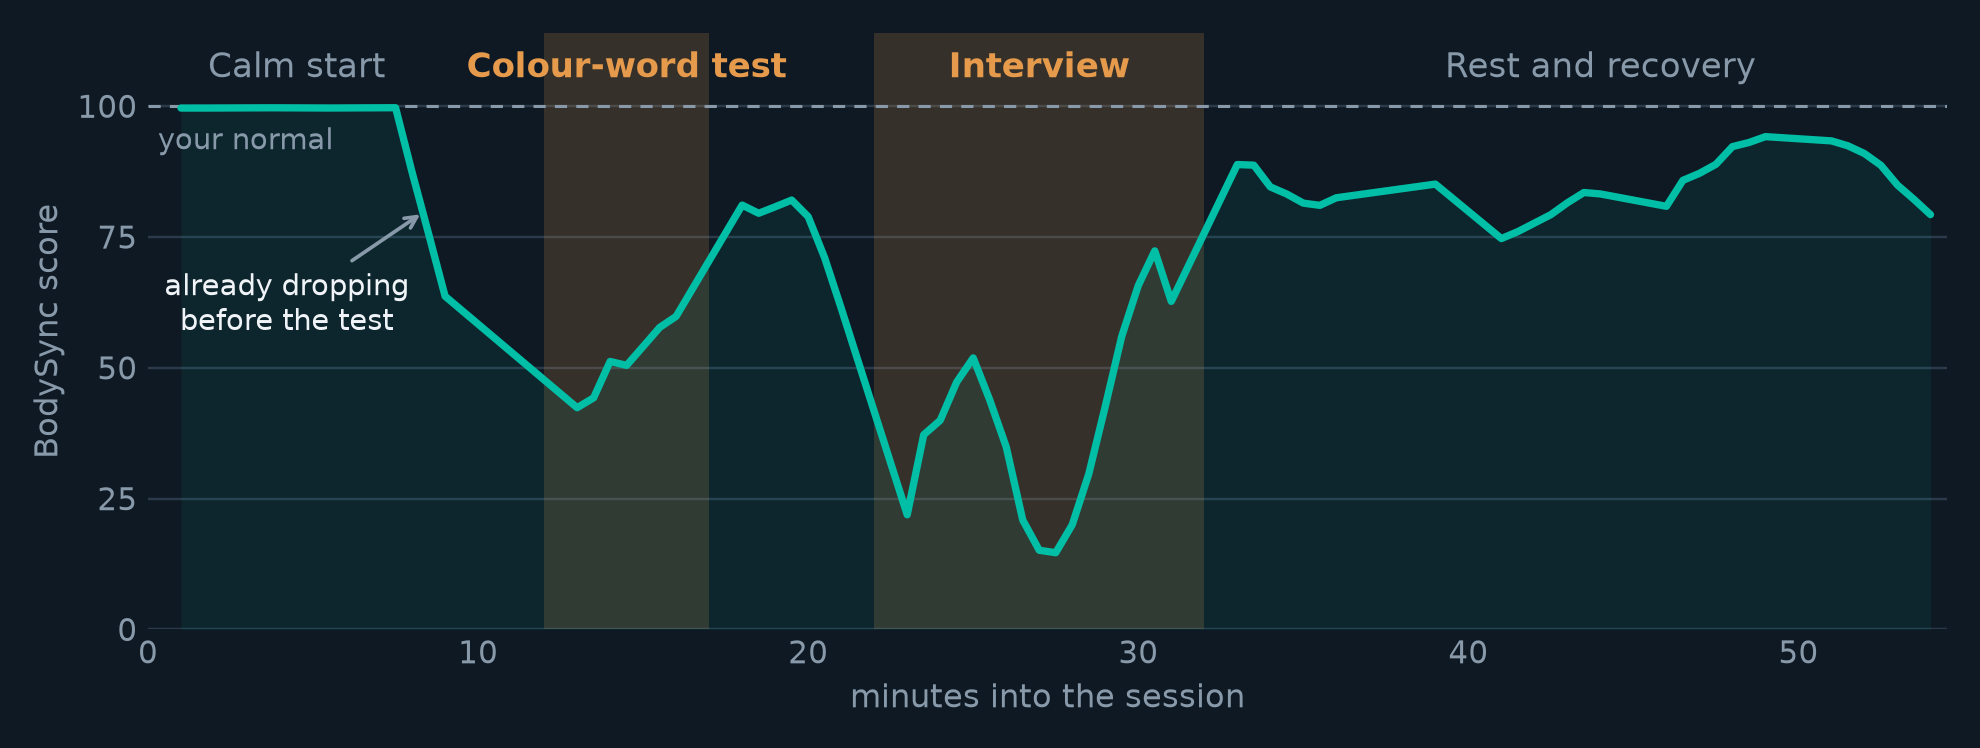
\includegraphics[width=0.9\linewidth]{fig7_example_person.png}
\caption{One locked test person from Stress-Predict, scored by the final BodySync. The score drops during both stress tasks and climbs back towards normal during rest. This is one of the clearer people; on average, stress is picked out about 9 times in 10.}
\end{figure}

\section{Takeaways}

\begin{itemize}
\item Comparing your signals with your own normal works; how they move together does not.
\item On lab stress, BodySync reaches about 0.9 or better on every dataset, on people it never saw (though lab timing cannot be fully ruled out).
\item On real roads it scores 0.76 for city vs highway with a model that never saw the dataset, and movement or timing cannot explain it.
\item In daily life it improves on the largest dataset; mild, self-reported everyday stress remains the hard part.
\end{itemize}

\section{Limitations}

\begin{itemize}
\item \textbf{Small test groups.} The daily-life result rests on 10 test people and the driving result on 9, so both are uncertain. Two smaller studies (nurse stress~\cite{nurse}, ADARP~\cite{adarp}) had only 4 test people each and scored near a coin flip; they are left out here but kept in the code repository.
\item \textbf{Lab timing.} In every lab study stress comes at the same point in the session, and a model given only the clock scores 0.78--0.97. BodySync never sees the clock, but lab data alone cannot rule out that it partly tracks time; the driving test, where time scores 0.50, is the main evidence against this.
\item \textbf{Everyday life.} Everyday stress is milder and rated only a few times a day. In CAN-STRESS the calm ratings cluster in the evening, so time of day may explain part of the gain from 0.59 to 0.67.
\item \textbf{The normal uses the whole recording.} Each person's normal is computed from all of their data, including later days; a real app would only have the past. A past-only normal was tried and did not help on the development people.
\item \textbf{Coarse in time.} BodySync tells stressful stretches from calm ones, but it does not follow moment-to-moment stress: on AffectiveROAD it hardly tracks the drivers' own continuous stress rating (correlation about 0.1).
\item \textbf{Self-training is a small, uneven gain.} It adds about 0.02 on average, mostly on real driving (0.08); on the lab studies it adds almost nothing.
\end{itemize}

Code and all results: \url{https://github.com/swaylakh/bodysync}

{\footnotesize
\begin{thebibliography}{9}
\setlength{\itemsep}{0pt}
\bibitem{sun2026trust} X.~Sun, R.~Ma, S.~Wei, P.~Cesar, J.~A.~Bosch, A.~El~Ali. Understanding trust toward human versus AI-generated health information through behavioral and physiological sensing. \emph{International Journal of Human-Computer Studies}, 209:103714, 2026.
\bibitem{wesad} P.~Schmidt, A.~Reiss, R.~D\"urichen, C.~Marberger, K.~Van~Laerhoven. Introducing WESAD, a multimodal dataset for wearable stress and affect detection. \emph{ICMI}, 2018.
\bibitem{stresspredict} T.~Iqbal et al. Stress monitoring using wearable sensors: a pilot study and Stress-Predict dataset. \emph{Sensors}, 22(21):8135, 2022.
\bibitem{stressexercise} A.~Hongn, F.~Bosch, L.~E.~Prado, J.~M.~Ferr\'andez~Vicente, M.~P.~Bonomini. Wearable physiological signals under acute stress and exercise conditions. \emph{Scientific Data}, 12:520, 2025.
\bibitem{nurse} S.~Hosseini et al. A multimodal sensor dataset for continuous stress detection of nurses in a hospital. \emph{Scientific Data}, 9:255, 2022.
\bibitem{adarp} R.~K.~Sah et al. ADARP: a multi modal dataset for stress and alcohol relapse quantification in real life setting. \emph{IEEE BSN}, 2022.
\bibitem{canstress} R.~Rahimi~Azghan et al. CAN-STRESS: a real-world multimodal dataset for understanding cannabis use, stress, and physiological responses. \emph{IEEE BSN}, 2025.
\bibitem{affectiveroad} N.~El~Haouij, J.-M.~Poggi, S.~Sevestre-Ghalila, R.~Ghozi, M.~Ja\"idane. AffectiveROAD system and database to assess driver's attention. \emph{ACM SAC}, 2018.
\end{thebibliography}
}

\end{document}
